
\chapter{Introduction}
\label{cha:introduction}

\texttt{PAFFS} stands for "Protective Aeronautics Flash FS" and aims to use a minimum RAM footprint with the ability to manage multiple flashes. Most of the design ideas are inspired by the filesystem \referenceDocument{JFFS3}, which was later extended (\referenceDocument{JFFS3ex]) and discontinued as predecessor of \texttt{UBIFS}.

\section{Fundamental structures}
\label{sec:funst}

\subsection{Areas}
\paragraph{Overview}
\begin{itemize}
	\item To separate between different Types of Data
	\item \texttt{AreaType} can be one of Superblock, Index, Data, (Journaling)
	\item Address split in \texttt{logical area n°} and \texttt{page n°}, to give way for an easy garbage collector (see  fig. \ref{fig:area_address})
	\item \texttt{AreaMap} held in FLASH (but cached in RAM) translates between \texttt{logical area n°} and \texttt{physical area n°}
	\item \texttt{AreaMap} also keeps record of corresponding types and usage statistics for garbage collection
\end{itemize}

\paragraph{AreaTypes}
\begin{itemize}
	\item[Superblock] Superblock is automatically first\footnote{\texttt{\textbf{or first two, just to be sure?}}} area of flash. It contains 
\end{itemize}


\section{Images}

\begin{figure}[ht]
  \centering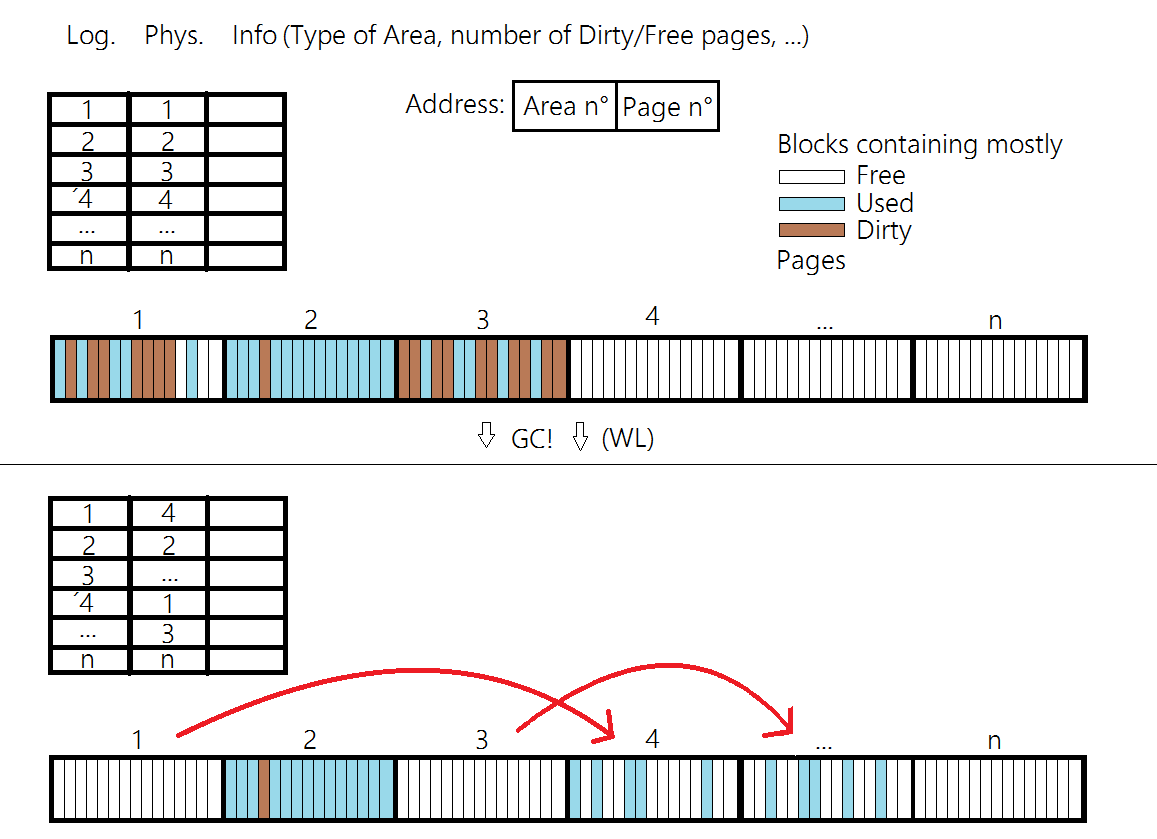
\includegraphics[width=\textwidth]{Areas_address.png}
  \caption{Basic process of garbage collection with areas}
  \label{fig:area_address}
\end{figure}
%
%\begin{figure}[htp]
%	\centering
%	\begin{subfigure}[t]{.49\textwidth}
%		\centering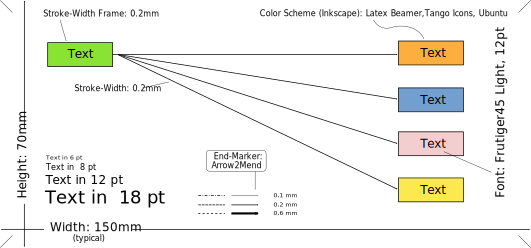
\includegraphics[width=7cm]{graphics_example}
%		\label{fig:graphics_example}
%		\subcaption{Example}
%	\end{subfigure}
%	\begin{subfigure}[t]{.49\textwidth}
%		\centering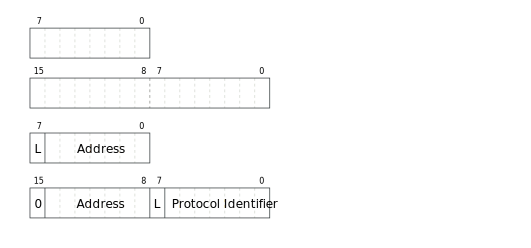
\includegraphics[width=7cm]{protocol_description_example}
%		\label{fig:protocol_example}
%		\subcaption{Protocol}
%	\end{subfigure}
%	\label{fig:images}
%	\caption{Two images side by side}
%\end{figure}


%\begin{lstlisting}[caption={Example C++ Code Listing},language=c++]
%enum TelemetryGeneration
%{
%    noTelemetry,
%    generateTelemetry
%};
%
%class Example
%{
%public:
%    Example(TelemetryGeneration telemetry,
%            uint8_t* buffer,
%            uint16_t length);
%    ...
%};
%
%Example object1(noTelemetry, 0, 0);
%
%uint8_t buffer[16];
%Example object1(generateTelemetry, buffer, size(buffer));
%\end{lstlisting}